\documentclass{UVA_ABNT}


%%%%%%%%%%%%%%%%%%%%%%%%%%%%%%%%%%%%%%%%%%%%%
%%%%%%%%%%%%% Imports Packages %%%%%%%%%%%%%%
%%%%%%%%%%%%%%%%%%%%%%%%%%%%%%%%%%%%%%%%%%%%%

\usepackage{times}              % Sets font to Times New Roman

\usepackage[utf8]{inputenc}     % Configures encoding to portuguese
\usepackage[T1]{fontenc}        % Configures encoding to portuguese  
\usepackage[portuguese]{babel}  % Configures encoding to portuguese
\usepackage{csquotes}
\usepackage{geometry}           % To adjust page layout
\usepackage{fancyhdr}           % For custom headers and footers
\usepackage[linktoc=all]{hyperref}           % For hyperlinks
\usepackage{bookmark}
\usepackage{tikz}               % For drawing diagrams 
\usepackage{enumitem}           % For customizing lists
\usepackage{graphicx}           % For including graphics 
\usepackage{changepage}
\usepackage{relsize}
\usepackage{indentfirst}        % Indents first paragraph
\usepackage{listings}           % For lists of things
% \usepackage[newfloat]{minted}   % For formated blocks of code
\usepackage{caption}
\usepackage{lipsum}
\usepackage{biblatex}       % For ABNT bibliography generation
\usepackage{tabularx}       % For multiple collumns 
\usepackage[explicit]{titlesec}
\usepackage{tocbasic}
\usepackage{setspace}


%%%%%%%%%%%%%%%%%%%%%%%%%%%%%%%%%%%%%%%%%%%%%
%%%%%%%% Configures Packages & Page %%%%%%%%%
%%%%%%%%%%%%%%%%%%%%%%%%%%%%%%%%%%%%%%%%%%%%%

% Configures biblatex
\addbibresource{Referencias.bib}
\AtBeginBibliography{\renewcommand*{\mkbibnamefamily}[1]{\textsc{#1}}}


% Sets lineheight
\renewcommand{\baselinestretch}{1.5} 

% Sets figure counter name
\renewcommand{\figurename}{Imagem}

% Creates color variable names
\definecolor{bgGrey}{rgb}{0.95,0.95,0.95}

% Configures table of contents name
\addto\captionsportuguese{%
  \renewcommand{\contentsname}%
    {\hfill SUMÁRIO \hfill}%
}

\DeclareTOCStyleEntries[
  linefill=\dotfill,
  numwidth=35pt,
  numsep=1ex,
  dynnumwidth,
  indent=0pt
]{tocline}{chapter,section,subsection,subsubsection}

\DeclareTOCStyleEntries[
    entryformat=\bfseries,
    entrynumberformat=\bfseries,
    pagenumberformat=\bfseries
]{tocline}{section, subsubsection}


% Configures minted
% \setminted{
% frame=lines,
% framesep=2mm,
% baselinestretch=1,
% bgcolor=bgGrey,
% fontsize=\footnotesize,
% linenos
% }

% \newenvironment{longlisting}{\captionsetup{type=listing}}{}
% \SetupFloatingEnvironment{listing}{name=Código}

% Definindo as margens
\geometry{top=3cm,bottom=2cm,left=3cm,right=2cm}

% Sets page style to show page numbering on header
\pagestyle{fancy}

\fancyhead{}
\setlength\headheight{26pt}
\fancyhead[L]{
\includegraphics[width=2cm]{Figuras/uva_header.png}}
\fancyhead[R]{\thepage}
\fancyfoot{}

\fancypagestyle{pretext}{%
    \fancyhf{}
    \setlength\headheight{26pt}
    \fancyhead[L]{
\includegraphics[width=2cm]{Figuras/uva_header.png}}
}

%  Edit section formating
\titleformat{\section}
    {\normalfont\bfseries}{\thesection}{1em}{\uppercase{#1}}

\titleformat{\subsection}
    {\normalfont}{\thesubsection}{1em}{\MakeUppercase{#1}}

\titleformat{\subsubsection}
  {\normalfont\bfseries}{\thesubsubsection}{1em}{{#1}}


%%%%%%%%%%%%%%%%%%%%%%%%%%%%%%%%%%%%%%%%%%%%%%
%%%%%%%%%%%%%% Valores do Documento %%%%%%%%%%
%%%%%%%%%%%%%%%%%%%%%%%%%%%%%%%%%%%%%%%%%%%%%%


\setTitle[Título do Trabalho em Portugues]
\setSubtitle[Subtítulo do Trabalho em Portugues]

\setCity[Rio de Janeiro]

\setAuthors[Vinicius DE AZEVEDO LIMA E SOUZA \\ 1240201902]


%%%%%%%%%%%%%%%%%%%%%%%%%%%%%%%%%%%%%%%%%%%%%
%%%%%%%%%%%%%% Document Body %%%%%%%%%%%%%%%%
%%%%%%%%%%%%%%%%%%%%%%%%%%%%%%%%%%%%%%%%%%%%%

\begin{document} 

    %%%%%%%% Elementos Externos %%%%%%%%%%

    \begin{titlepage}
    
    \centering
    
    \begin{figure}[h]
        \centering
        
\includegraphics[width=1.8cm]{Figuras/uva.png}
    \end{figure}
        
    \textbf{
        \uppercase{
            Universidade Veiga de Almeida \\
            Ciência da Computação
        }
    }
    %\textbf{NOME DO DEPARTAMENTO} \\
    \vspace{5 em}

    % Autores
    \printAuthors
    
    
    \vfill

    % Titulo do Trabalho
    \textbf{\uppercase\expandafter{\expanded{\TitleName}:}} \\
    \SubtitleName
    
        
    \vfill 
        
    % Local (cidade)
    \printCity \\
    \the \year

\end{titlepage}
 %% Página obrigatória
    
    %%%%%%%% Elementos Pré-Textuais

    %%%%%%%%%%%%%%%%%%%%%%%%%%%%%%%%%%%%%%%%%%%%%%
%%%%%%%%%%%% Página obrigatória %%%%%%%%%%%%%%
%%%%%%%%%%%%%%%%%%%%%%%%%%%%%%%%%%%%%%%%%%%%%%

\begin{center}

    \thispagestyle{pretext}
    \ \\ 

    \begin{large}
        \printAuthors
    \end{large}
    

    \vfill

    \begin{Large}
        \textbf{\uppercase\expandafter{\TitleName}:} \\
        \textbf{\uppercase\expandafter{\SubtitleName}}
    \end{Large}

\end{center}

\vspace{3em}

\begin{adjustwidth}{7.5cm}{}
    \noindent texto longo explicando o trabalho Lorem ipsum dolor sit amet, consectetur adipisci elit, sed eiusmod tempor incidunt ut labore et dolore magna aliqua. Ut enim ad minim veniam, quis nostrum exercitationem ullam corporis suscipit laboriosam, nisi ut aliquid ex ea commodi consequatur. Quis aute iure reprehenderit in voluptate velit esse cillum dolore eu fugiat nulla pariatur. Excepteur sint obcaecat cupiditat non proident, sunt in culpa qui officia deserunt mollit anim id est laborum. \\ \ \\
    Orientador: Prof Professor Nome
\end{adjustwidth}

\vfill

\begin{center}
    \begin{large}
        \printCity \\
        \the \year
    \end{large}
\end{center}

\newpage %% Página obrigatória

    %%%%%%%%%%%%%%%%%%%%%%%%%%%%%%%%%%%%%%%%%%%%%%
%%%%%%%%%%%% Página obrigatória %%%%%%%%%%%%%%
%%%%%%%%%%%%%%%%%%%%%%%%%%%%%%%%%%%%%%%%%%%%%%

\begin{center}

    \thispagestyle{pretext}
    
    \ \\ 
    \printAuthors

    \vfill

    \textbf{\uppercase\expandafter{\TitleName}:} \\
    \textbf{\uppercase\expandafter{\SubtitleName}}

    \vfill


    \begin{adjustwidth}{7.5cm}{}
        \noindent Trabalho de conclusão de curso, apresentado como requisito parcial para obtenção do título de Bacharel em Ciência da Computação pela Universidade Veiga de Almeida.
    \end{adjustwidth}

    \vfill

    {
        \setstretch{1}

        APROVADO EM\\[2cm]

        BANCA EXAMINADORA: \\[1.5cm]

        \rule{0.7\textwidth}{0.4pt} \\
        Prof. Nome \\ 
        UNIVERSIDADE VEIGA DE ALMEIDA \\[1.5cm]

        \rule{0.7\textwidth}{0.4pt} \\
        Prof. Nome \\ 
        UNIVERSIDADE VEIGA DE ALMEIDA \\[1.5cm]

        \rule{0.7\textwidth}{0.4pt} \\
        Prof. Nome \\ 
        UNIVERSIDADE VEIGA DE ALMEIDA \\
    }


\end{center}


\newpage
 %% Página obrigatória

    %%%%%%%%%%%%%%%%%%%%%%%%%%%%%%%%%%%%%%%%%%%%%%
%%%%%%%%%%%%% Página opcional %%%%%%%%%%%%%%%%
%%%%%%%%%%%%%%%%%%%%%%%%%%%%%%%%%%%%%%%%%%%%%%
\thispagestyle{pretext}

\vspace*{\fill}

\begin{flushright}
    Para meus pais, Mãe e Pai; \\
    e meus amigos, fulano, fulano e fulano. \\
    Eu não conseguiria sem vocês. \\
\end{flushright}

\newpage %% Página opcional

    %%%%%%%%%%%%%%%%%%%%%%%%%%%%%%%%%%%%%%%%%%%%%%
%%%%%%%%%%%%% Página opcional %%%%%%%%%%%%%%%%
%%%%%%%%%%%%%%%%%%%%%%%%%%%%%%%%%%%%%%%%%%%%%%
\thispagestyle{pretext}

\section*{\centering AGRADECIMENTOS}

\lipsum[2] \\

\lipsum[2] \\

\lipsum[2] \\

\newpage %% Página opcional

    %%%%%%%%%%%%%%%%%%%%%%%%%%%%%%%%%%%%%%%%%%%%%%
%%%%%%%%%%%%% Página opcional %%%%%%%%%%%%%%%%
%%%%%%%%%%%%%%%%%%%%%%%%%%%%%%%%%%%%%%%%%%%%%%
 %% Página opcional

    %%%%%%%%%%%%%%%%%%%%%%%%%%%%%%%%%%%%%%%%%%%%%%
%%%%%%%%%%%% Página obrigatória %%%%%%%%%%%%%%
%%%%%%%%%%%%%%%%%%%%%%%%%%%%%%%%%%%%%%%%%%%%%%
\thispagestyle{pretext}

\section*{\centering RESUMO}

\lipsum[3] \\

\noindent\textbf{Palavras-chave:} Palavra. Palavra. Palavra. Palavra. Palavra.

\newpage %% Página obrigatória

    %%%%%%%%%%%%%%%%%%%%%%%%%%%%%%%%%%%%%%%%%%%%%%
%%%%%%%%%%%% Página obrigatória %%%%%%%%%%%%%%
%%%%%%%%%%%%%%%%%%%%%%%%%%%%%%%%%%%%%%%%%%%%%%
 %% Página obrigatória
    
    \thispagestyle{pretext}
    \tableofcontents
    \newpage

    %%%%%%%%% Elementos Textuais
    

    \section{INTRODUÇÃO}

\lipsum[3] 

\newpage

    \section{Desenvolvimento}

\subsection{Formatação dos Títulos}

\begin{itemize}
    \item Título primário: Caixa alta e negritoç
    \item Título secundário: Caixa alta;
    \item Título terciário: Negrito;
    \item Título quaternário: ''Normal'';
    \item Título sem indicativos numéricos: Caixa alta, negrito, centralizado;
\end{itemize}

Títulos que ocupem mais de uma linha devem ser, a partir da segunda linha, alinhados abaixo da primeira letra da primeira palavra do título.

\subsubsection{Exemplo de titulo terciário}

\lipsum[2]

\subsection{Regras para o sumário}

\begin{figure}[h]
    \centering
    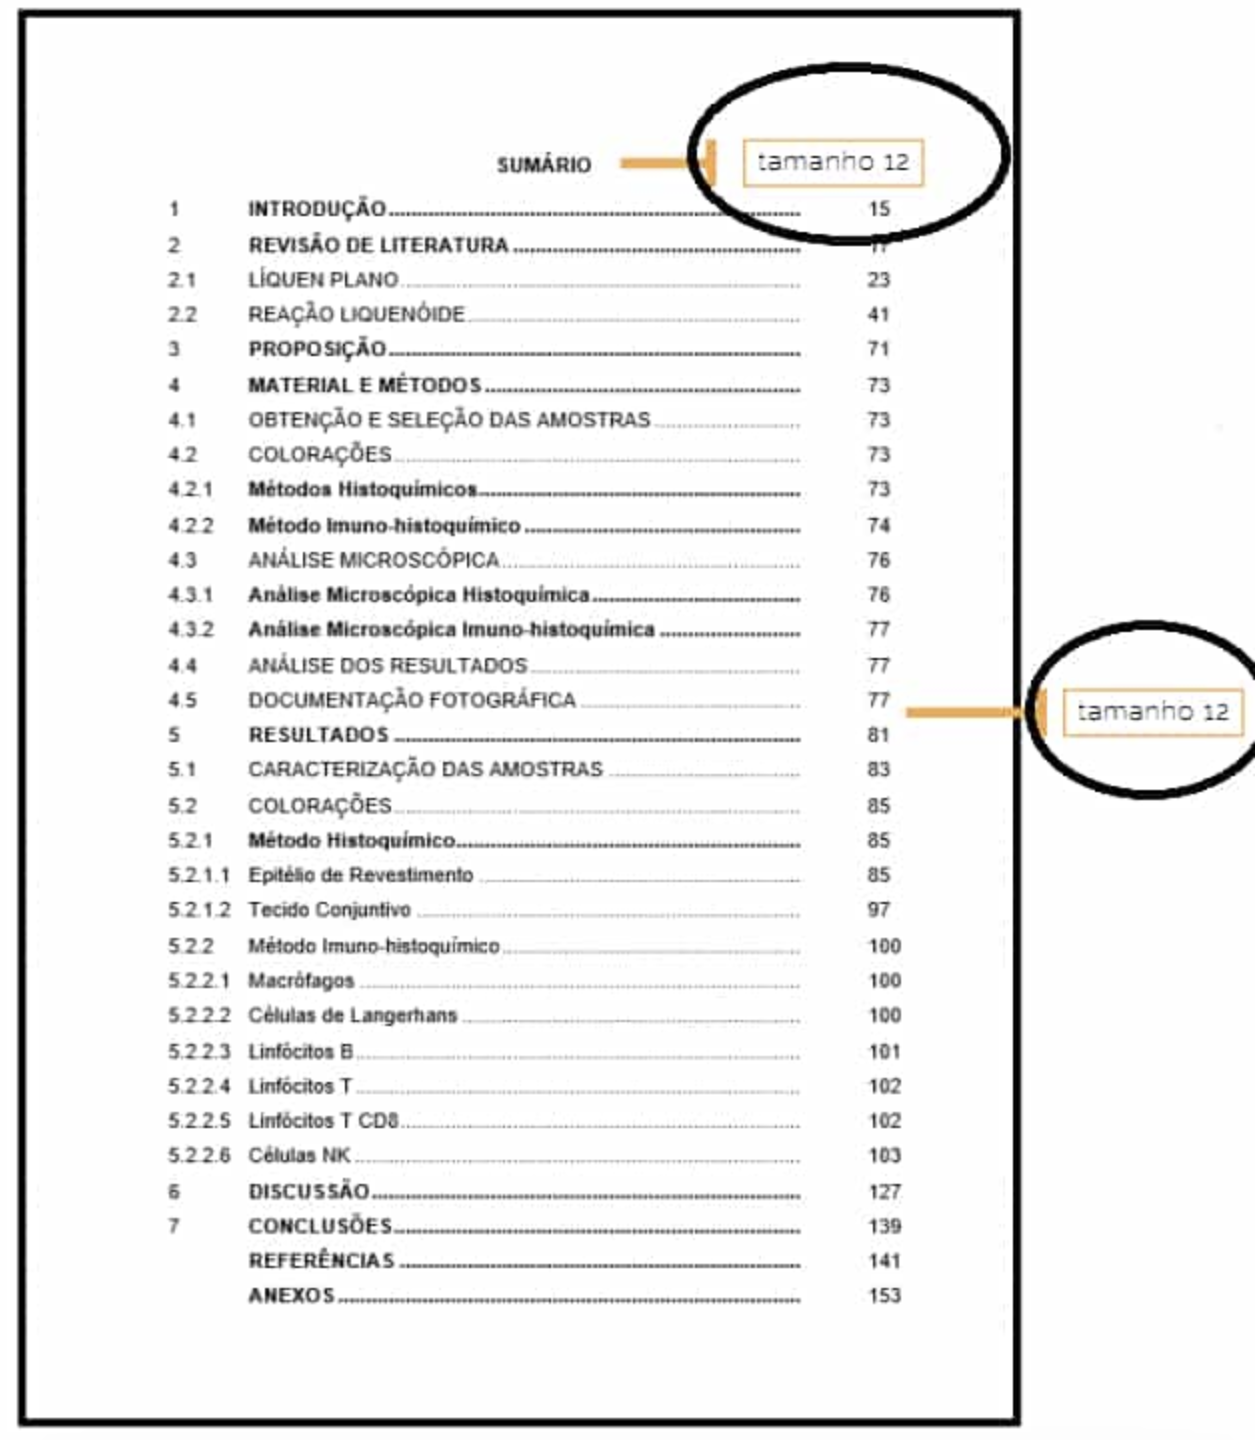
\includegraphics[width=0.9\textwidth]{Figuras/exemplo_sumario.png} % Change to the path of your image
    \caption{Exemplo de um sumário.}
    \label{fig:exemplo_sumario}
\end{figure}

\begin{itemize}
    \item A margem superior e esquerda deverá ser de 3 cm;
    \item A margem inferior e direita deverá ser de 2 cm;
    \item O título deverá ficar centralizado e em letra maiúscula;
    \item O sumário deverá ficar antes da introdução;
    \item Você deverá organizar de acordo com os capítulos, seções e partes, tudo na ordem que seu trabalho será!
    \item O sumário deverá ficar depois da capa, folha de rosto, folha de aprovação, dedicatória, resumo ou listas;
    \item A palavra “sumário” ficará no topo da página em negrito, com a mesma fonte e tamanho do resto do texto;
    \item O espaçamento entre as linhas deverá ser de 1,5;
    \item O tamanho da fonte deverá ser 12;
    \item Não deverão conter outros textos, apenas os títulos das divisões e subdivisões;
    \item Os capítulos devem ser escritos com todas as letras em caixa alta, com fonte tamanho 12, em negrito e em alinhamento à esquerda;
    \item Os subcapítulos devem ter a mesma formatação dos capítulos, mas com apenas a primeira letra maiúscula, o resto em letra minúscula;
    \item Os subcapítulos não são em negrito como os capítulos.
\end{itemize}


\subsection{Problem Statement Title}
\textbf{Problem:} Write the problem statement here. You can describe the problem in detail, such as equations, diagrams, or concepts involved.

\vspace{1em} % Adds space between problem and solution

\textbf{Solution:} Here, write your solution to the problem. This can include the following steps:
\begin{itemize}
    \item Step 1: Description or calculation.
    \item Step 2: Description or calculation.
    \item Step 3: Final solution or conclusion.
\end{itemize}

You can use mathematical formatting, such as:
\[
f(x) = \int_{0}^{\infty} e^{-x^2} \, dx
\]
or numbered equations like:
\begin{equation}
    E = mc^2
\end{equation}

\newpage

\subsection{Problem 2: Another Problem Title}
\textbf{Problem:} Another problem statement goes here.

\vspace{1em}

\textbf{Solution:} Another solution explanation with steps:
\begin{itemize}
    \item Step 1: Explanation.
    \item Step 2: Further solution.
\end{itemize}

You can also include diagrams or plots, for example:
\begin{figure}[h]
    \centering
    \includegraphics[width=0.5\textwidth]{example-image} % Change to the path of your image
    \caption{A sample diagram.}
    \label{fig:sample-diagram}
\end{figure}

\newpage

\subsection{Fazendo referncias bibliograficas}

% Para fazer referencias bibliograficas em LaTex, voce deve usar o comando \cite{dirac} para fazer uma citação à algum artigo mencionado no arquivo \texttt{Referencias.bib}.

% \cite{website:ArduinoLabview}
% \cite{website:OPENSOURCESW}
% \cite{website:OPENSOURCEHW}

\lipsum[3]

\section*{Abstratos}

\lipsum[3]

\newpage

    \section{CONCLUSÃO}

\lipsum[3]

\newpage

    %%%%%%%% Elementos Pós-Textuais

    \newpage
    \nocite{*}
    % \printbibliography[heading=bibintoc]

\end{document}
